\documentclass[14pt,a4paper,report]{report}
\usepackage[a4paper, mag=1000, left=2.5cm, right=1cm, top=2cm, bottom=2cm, headsep=0.7cm, footskip=1cm]{geometry}
\usepackage[utf8]{inputenc}
\usepackage[english,russian]{babel}
\usepackage{indentfirst}
\usepackage[dvipsnames]{xcolor}
\usepackage[colorlinks]{hyperref}
\usepackage{listings} 
\usepackage{fancyhdr}
\usepackage{caption}
\usepackage{graphicx}
\hypersetup{
	colorlinks = true,
	linkcolor  = black
}

\usepackage{titlesec}
\titleformat{\chapter}
{\Large\bfseries} % format
{}                % label
{0pt}             % sep
{\huge}           % before-code


\DeclareCaptionFont{white}{\color{white}} 

% Listing description
\usepackage{listings} 
\DeclareCaptionFormat{listing}{\colorbox{gray}{\parbox{\textwidth}{#1#2#3}}}
\captionsetup[lstlisting]{format=listing,labelfont=white,textfont=white}
\lstset{ 
	% Listing settings
	inputencoding = utf8,			
	extendedchars = \true, 
	keepspaces = true, 			  	 % Поддержка кириллицы и пробелов в комментариях
	language = C++,            	 	 % Язык программирования (для подсветки)
	basicstyle = \small\sffamily, 	 % Размер и начертание шрифта для подсветки кода
	numbers = left,               	 % Где поставить нумерацию строк (слева\справа)
	numberstyle = \tiny,          	 % Размер шрифта для номеров строк
	stepnumber = 1,               	 % Размер шага между двумя номерами строк
	numbersep = 5pt,              	 % Как далеко отстоят номера строк от подсвечиваемого кода
	backgroundcolor = \color{white}, % Цвет фона подсветки - используем \usepackage{color}
	showspaces = false,           	 % Показывать или нет пробелы специальными отступами
	showstringspaces = false,    	 % Показывать или нет пробелы в строках
	showtabs = false,           	 % Показывать или нет табуляцию в строках
	frame = single,              	 % Рисовать рамку вокруг кода
	tabsize = 2,                  	 % Размер табуляции по умолчанию равен 2 пробелам
	captionpos = t,             	 % Позиция заголовка вверху [t] или внизу [b] 
	breaklines = true,           	 % Автоматически переносить строки (да\нет)
	breakatwhitespace = false,   	 % Переносить строки только если есть пробел
	escapeinside = {\%*}{*)}      	 % Если нужно добавить комментарии в коде
}

\begin{document}

\def\contentsname{Содержание}

% Titlepage
\begin{titlepage}
	\begin{center}
		\textsc{Санкт-Петербургский Политехнический 
			Университет Петра Великого\\[5mm]
			Кафедра компьютерных систем и программных технологий}
		
		\vfill
		
		\textbf{Отчёт по лабораторной работе №1\\[3mm]
			Курс: «Системное программирование»\\[6mm]
			Тема: «Обработка исключений в ОС Windows»\\[35mm]
		}
	\end{center}
	
	\hfill
	\begin{minipage}{.4\textwidth}
		Выполнил студент:\\[2mm] 
		Бояркин Никита Сергеевич\\
		Группа: 13541/3\\[5mm]
		
		Проверил:\\[2mm] 
		Душутина Елена Владимировна
	\end{minipage}
	\vfill
	\begin{center}
		Санкт-Петербург\\ \the\year\ г.
	\end{center}
\end{titlepage}

% Contents
\tableofcontents
\clearpage

\chapter{Лабораторная работа №1}

\section{Цель работы}

Научиться обрабатывать исключения с помощью встроенных средств WinAPI. Использовать системные утилиты для получения информации о системной активности процесса.

\section{Программа работы}

\begin{enumerate}
	\item Сгенерировать и обработать исключения с помощью функций WinAPI;
	\item Получить код исключения с помощью функции GetExceptionCode.
	\begin{itemize}
		\item Использовать эту функции в выражении фильтре;
		\item Использовать эту функцию в обработчике.
	\end{itemize}
	\item Создать собственную функцию-фильтр;
	\item Получить информацию об исключении с помощью функции GetExceptionInformation; сгенерировать исключение с помощью функции RaiseException;
	\item Использовать функции UnhandleExceptionFilter и Set UnhandleExceptionFilter для необработанных исключений;
	\item Обработать вложенные исключения;
	\item Выйти из блока \_\_try с помощью оператора goto;
	\item Выйти из блока \_\_try с помощью оператора leave;
	\item Преобразовать структурное исключение в исключение языка С, используя функцию translator;
	\item Использовать финальный обработчик finally;
	\item Проверить корректность выхода из блока \_\_try с помощью функции AbnormalTermination в финальном обработчике finally.
\end{enumerate}

\clearpage

\section{Характеристики системы}

Некоторая информация об операционной системе и ресурсах системы:

\begin{figure}[h!]
	\centering
	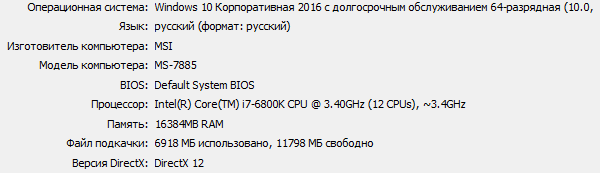
\includegraphics[scale = 1.05]{images/0_s.png}
	\caption{Конфигурация системы}
\end{figure}

Информация о компиляторе:

\lstinputlisting{listings/0.c.log}

Информация о компоновщике:

\lstinputlisting{listings/0.l.log}

Версии используемых утилит:

\begin{figure}[h!]
	\centering
	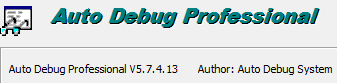
\includegraphics[scale = 1.15]{images/0_d.png}
	\caption{Версия утилиты Auto Debug}
\end{figure}

\begin{figure}[h!]
	\centering
	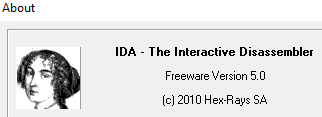
\includegraphics[scale = 1.15]{images/0_i.png}
	\caption{Версия деассемблера Ida}
\end{figure} 

\clearpage

\section{Ход работы}

\subsection{Генерация и обработка исключения средствами WinAPI}

В операционной системе Windows используется  механизм структурной обработки исключений (SEH). В отличие от встроенных средств обработки исключений языка C++, SEH позволяет обрабатывать не только программные исключения, но и аппаратные.

\lstinputlisting{listings/1.t.cpp}

Если при выполнении защищенного кода из блока \_\_try возникнет исключение, то операционная система перехватит его и приступит к поиску блока \_\_except. Найдя его, она передаст управление фильтру исключений. Фильтр исключений может получить код исключения и на основе этого кода принять решение, передать управление обработчику или же сказать системе, чтобы она искала предыдущий по вложенности блок \_\_except [1] Фильтр исключений может возвращать одно из трех значений (идентификаторов), которые определены в файле excpt.h:

\begin{itemize}
	\item Идентификатор EXCEPTION\_EXECUTE\_HANDLER означает, что для этого блока \_\_try есть обработчик исключения и он готов обработать это исключение.
	\item Идентификатор EXCEPTION\_CONTINUE\_SEARCH означает, что для обработки исключения существует предыдущий по вложенности блок \_\_except.
	\item Идентификатор EXCEPTION\_CONTINUE\_EXECUTION означает, что выполнение продолжится с того участка кода, который вызвал исключение.
\end{itemize}

Подобная система обработки исключений позволяет организовывать вложенные исключения, что значительно увеличивает гибкость и читабельность языка программирования.

Некоторые типы исключений, которые могут быть обработаны в фильтре [2]:

\begin{itemize}
	\item EXCEPTION\_ACCESS\_VIOLATION -- попытка чтения или записи в виртуальную память без соответствующих прав доступа;
	\item EXCEPTION\_BREAKPOINT -- встретилась точка останова;
	\item EXCEPTION\_DATATYPE\_MISALIGNMENT -- доступ к данным, адрес которых не выровнен по границе слова или двойного слова;
	\item EXCEPTION\_SINGLE\_STEP -- механизм трассировки программы сообщает, что выполнена одна инструкция;
	\item EXCEPTION\_ARRAY\_BOUNDS\_EXCEEDED -- выход за пределы массива, если аппаратное обеспечение поддерживает такую проверку;
	\item EXCEPTION\_FLT\_DENORMAL\_OPERAND -- один из операндов с плавающей точкой является ненормализованным;
	\item EXCEPTION\_FLT\_DIVIDE\_BY\_ZERO -- попытка деления на ноль в операции с плавающей точкой;
	\item EXCEPTION\_FLT\_INEXACT\_RESULT -- результат операции с плавающей точкой не может быть точно представлен десятичной дробью;
	\item EXCEPTION\_FLT\_INVALID\_OPERATION -- ошибка в операции с плавающей точкой, для которой не предусмотрены другие коды исключения;
	\item EXCEPTION\_FLT\_OVERFLOW -- при выполнении операции с плавающей точкой произошло переполнение;
	\item EXCEPTION\_FLT\_STACK\_CHECK -- переполнение или выход за нижнюю границу стека при выполнении операции с плавающей точкой;
	\item EXCEPTION\_FLT\_UNDERFLOW -- результат операции с плавающей точкой является числом, которое меньше минимально возможного числа с плавающей точкой;
	\item EXCEPTION\_INT\_DIVIDE\_BY\_ZERO -- попытка деления на ноль при операции с целыми числами;
	\item EXCEPTION\_INT\_OVERFLOW -- при выполнении операции с целыми числами произошло переполнение;	
	\item EXCEPTION\_PRIV\_INSTRUCTION -- попытка выполнения привилегированной инструкции процессора, которая недопустима в текущем режиме процессора;
	\item EXCEPTION\_NONCONTINUABLE\_EXCEPTION -- попытка возобновления исполнения программы после исключения, которое запрещает выполнять такое действие.
\end{itemize}

Разработаем программу, которая генерирует исключение EXCEPTION\_INT\_DIVIDE\_BY\_ZERO из защищенного участка кода и выводит его шестнадцатиричный код в обработчике:

\lstinputlisting{listings/1.z.cpp}

Результат работы программы:

\lstinputlisting{listings/1.z.log}

Попробуем обработать аппаратное исключение EXCEPTION\_FLT\_OVERFLOW:

\lstinputlisting{listings/1.f.cpp}

Результат работы программы:

\lstinputlisting{listings/1.f.log}

Оба исключения были успешно обработаны. В качестве фильтра для обработчика был использован простой тернарный оператор, который вызывает обработчик только при возникновении конкретного исключения. Если исключение не было вызвано, то поиск обработчика продолжится, что для данного случая эквивалентно падению программы.

Для получения более детальной информации о поведении системы при обработке исключений, рассмотрим последовательность произведенных системных вызовов. 

\clearpage

\begin{figure}[h!]
	\centering
	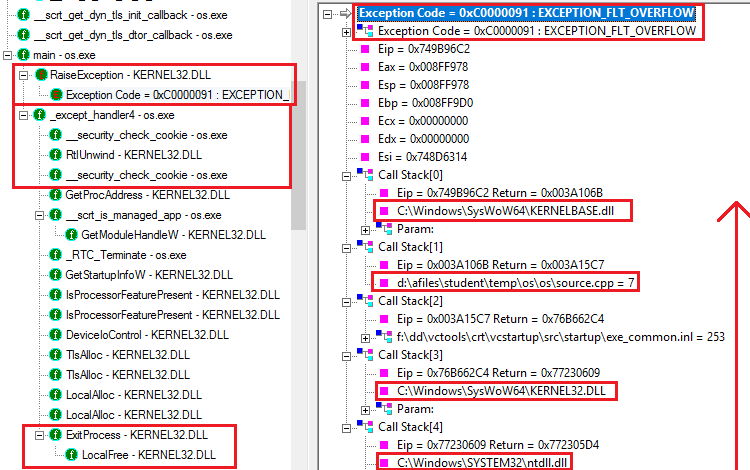
\includegraphics[scale = 0.69]{images/1.png}
	\caption{Системные вызовы в программе обработки исключения EXCEPTION\_FLT\_OVERFLOW}
\end{figure}

После подготовительной стадии запуска процесса вызывается функция main. Первой выполняемой инструкцией данной программы является обращение к библиотеке ядра Windows KERNEL32.DLL функцией RaiseException. В результате выбрасывается исключение с кодом 0xC0000091 (EXCEPTION\_FLT\_OVERFLOW). Стек вызовов, производимых при выбрасывании исключения продемонстрирован на рисунке 1.4. 

Все последующие операции производятся уже в обработчике исключения (\_except\_handler4). Стоит отметить, что в первую очередь производится \textbf{раскрутка стека} (RtlUnwind) -- процесс, в результате которого программа последовательно покидает составные инструкции и определения функций в поисках обработчика, способного обработать возникшее исключение [3]. По мере раскрутки прекращают существование локальные объекты, объявленные в составных инструкциях и определениях функций, из которых произошел выход.

\subsubsection{Иллюстрация процесса обработки исключения в деассемблере Ida}

Рассмотрим процесс генерации исключения и раскрутки стека подробнее. Ida позволяет получить деассемблированную версию программы с возможностью осуществления пошаговой отладки, просмотра регистров процессора, просмотра кода внешних функций и др. 

После прохождения всех подготовительных стадий вызывается главная функция main, из которой вызывается внешняя функция ядра RaiseException с тремя нулевыми аргументами и кодом исключения (0xC0000091 EXCEPTION\_FLT\_OVERFLOW):

\begin{figure}[h!]
	\centering
	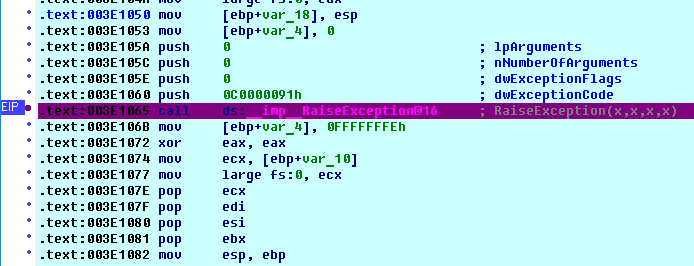
\includegraphics[scale = 0.85]{images/1_d1.png}
	\caption{Вызов внешней функции RaiseException из функции main}
\end{figure}

Стоит отметить, что последющий код функции main соответствует нормальному выходу из охраняемого кода, то есть случаю, когда исключение не сгенерируется. В нашем случае эта ветка кода не будет вызвана.

Как и следовало ожидать, было сгенерировано исключение EXCEPTION\_FLT\_OVERFLOW:

\begin{figure}[h!]
	\centering
	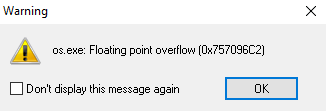
\includegraphics[scale = 0.69]{images/1_d2.png}
	\caption{Уведомление о произошедшем исключении}
\end{figure}

После этого вызывается функция фильтр, которая проверяет код исключения на совпадение с 0xC0000091:

\begin{figure}[h!]
	\centering
	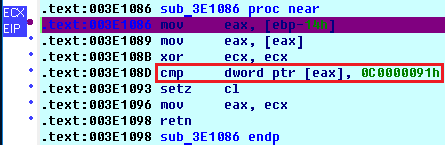
\includegraphics[scale = 0.75]{images/1_d3.png}
	\caption{Функция фильтр}
\end{figure}

После этого последовательно вызываются дорогостоящие функции раскрутки стека RtlUnwind в модулях ядра kernel32 и ntdll:

\begin{figure}[h!]
	\centering
	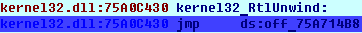
\includegraphics[scale = 0.95]{images/1_d5.png}
	\caption{Функция раскрутки стека RtlUnwind в модуле kernel32}
\end{figure}

\begin{figure}[h!]
	\centering
	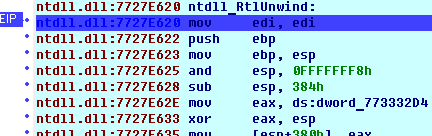
\includegraphics[scale = 0.75]{images/1_d6.png}
	\caption{Функция раскрутки стека RtlUnwind в модуле ntdll}
\end{figure}

Количество ассемблерных команд в RtlUnwind достаточно большое, что подтверждает ожидания. 

Так как фильтр сработал, вызывается код обработчика, вызывающий внешнюю функцию вывода сообщения на экран:

\begin{figure}[h!]
	\centering
	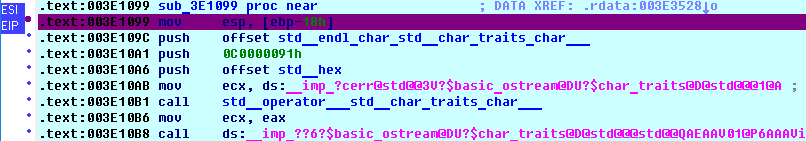
\includegraphics[scale = 0.75]{images/1_d4.png}
	\caption{Код обработчика исключения}
\end{figure}


\subsection{Получить код исключения с помощью функции GetExceptionCode}

\subsubsection{Использовать эту функцию в выражении фильтре}

Для получения кода выброшенного исключения, вызывается функция GetExceptionCode, имеющая следующий прототип:

\begin{lstlisting}
DWORD GetExceptionCode(void);
\end{lstlisting}

Функцию можно вызывать внутри фильтра, а также непосредственно внутри обработчика исключения. Правилом хорошего тона при программировании является явное указание в фильтре всех возможных для данного охраняемого кода исключений. Таким образом те исключения, о которых программист не подумал дадут о себе знать на этапе отладки.

Разработаем программу, которая использует функцию GetExceptionCode внутри тернарного оператора фильтра:

\lstinputlisting{listings/2.1.z.cpp}

Результат работы программы:

\lstinputlisting{listings/2.1.z.log}

По умолчанию аппаратные исключения, связанные с числами с плавающей точкой, не нуждаются в обработке. Для того, чтобы явно указать необходимость обработки исключений с плавающей точкой, разработаем функцию activateFloatExceptions:

\lstinputlisting{listings/2.1.f.cpp}

Результат работы программы:

\lstinputlisting{listings/2.1.f.log}

Таким образом, средствами WinAPI можно обрабатывать не только программные исключения, а также аппаратные, которые игнорируются по-умолчанию.

\subsubsection{Использовать эту функцию в обработчике}

Использование функции GetExceptionCode возможно также непосредственно внутри обработчика, однако, не стоит подменять фильтр этой возможностью, особенно при работе со вложенными исключениями.

Разработаем программу, получающую код исключения непосредственно внутри обработчика:

\lstinputlisting{listings/2.2.z.cpp}

Результат работы программы:

\lstinputlisting{listings/2.2.z.log}

Теперь разработаем аналогичную программу для исключения с плавающей точкой:

\lstinputlisting{listings/2.2.f.cpp}

Результат работы программы:

\lstinputlisting{listings/2.2.f.log}

В результате эксперимента было выявлено, что функция GetExceptionCode выдает корректный результат при вызове непосредственно внутри обработчика.

\subsection{Создать собственную функцию-фильтр}

Для больших программ, в которых использование фильтрующего тернарного оператора недостаточно, функциональность фильтра бывает удобно перенести во внешнюю функцию. При этом данная функция должна возвращать один из трех идентификаторов, определяющих поведение программы.

Разработаем программу с отдельной фильтрующей функцией:

\lstinputlisting{listings/3.z.cpp}

Результат работы программы аналогичен фильтру с тернарным оператором:

\lstinputlisting{listings/3.z.log}

Модифицируем программу, порождающую исключение переполнения числа с плавающей точкой. Программист пытается сгенерировать очень большое число функцией возведения в степень, однако, натыкается на переполнение в охраняемом коде. Функция фильтр фиксирует это исключение и изменяет эту переменную на другое очень большое число, после чего продолжает выполнение программы. Все остальные исключения обрабатываются непосредственно внутри обработчика.

\lstinputlisting{listings/3.f.cpp}

Результат работы программы:

\lstinputlisting{listings/3.f.log}

Исключение было выброшено внутри функции возведения в степень. После чего была вызвана функция фильтра. Значение переменной не было перезаписано, так как исключение было выброшено до этого. Затем внутри фильтра значение переменной перезаписывается и блок охраняемого кода нормально завершается.

\subsection{Получить информацию об исключении, сгенерировать исключение}

Помимо функции GetExceptionCode внутри фильтра или обработчика можно вызвать функцию GetExceptionInformation, которая возвращает заполненную структуру, в полях которой содержится детальная информация об исключении. Сигнатура функции выглядит следующим образом:

\begin{lstlisting}
LPEXCEPTION_POINTERS GetExceptionInformation(void);
\end{lstlisting}

Возвращаемая структура содержит указатели на структуру EXCEPTION\_RECORD и на структуру CONTEXT. Структура EXCEPTION\_RECORD содержит машинно-независимое описание исключения, CONTEXT содержит специфическое состояние процессора на момент исключения [4]

В большинстве случаев интересующая программиста информация содержится в структуре EXCEPTION\_RECORD, со следующими полями:

\begin{itemize}
	\item ExceptionCode -- код исключения, совпадающий с результатом функции GetExceptionCode.
	\item ExceptionFlags -- флаги исключения.
	\item ExceptionAddress -- адрес, по которому было вызвано исключение.
	\item NumberParameters -- количество элементов массива ExceptionInformation.
	\item ExceptionInformation -- массив, содержащий наиболее детальную информацию о исключении. Может быть задан функцией RaiseException, а также определен для специфических исключений (например EXCEPTION\_ACCESS\_VIOLATION). В остальных случаях массив не определен.
	\item ExceptionRecord -- указатель на связанную структуру EXCEPTION\_RECORD.
\end{itemize}

Исключение можно сгенерировать функцией RaiseException со следующей сигнатурой [5]:

\begin{lstlisting}
void WINAPI RaiseException(
    _In_       DWORD     dwExceptionCode,
    _In_       DWORD     dwExceptionFlags,
    _In_       DWORD     nNumberOfArguments,
    _In_ const ULONG_PTR *lpArguments
);
\end{lstlisting}

В качестве параметров обязательно указывается код исключения, который может быть собственным. Необязательными параметрами являются флаги исключения, а также массив детализированной информации с указанием количества аргументов.

Разработаем фильтрующую функцию, которая записывает в глобальную переменную информацию о последнем возникшем исключении, после чего в обработчике использует эти данные, если необходимо:

\lstinputlisting{listings/4.z.cpp}

Результат работы программы:

\lstinputlisting{listings/4.z.log}

Разработаем аналогичную программу для исключения EXCEPTION\_FLT\_OVERFLOW:

\lstinputlisting{listings/4.f.cpp}

Результат работы программы:

\lstinputlisting{listings/4.f.log}

Таким образом, для простых исключений с целыми и нецелыми числами поля ExceptionFlags, ExceptionRecord и ExceptionInformation не определены. Это объясняется тем, что как правило такие исключения простые и не требуют каких либо дополнительных пояснений.

Рассмотрим стек вызовов при генерации исключения деления на ноль. Видно, что последний вызов, породивший исключение, имеет адрес 0x749B96C2 (поле Eip), что совпадает с информацией полученной в результате GetExceptionInformation. Более подробное описание регистров процессора находится в структуре CONTEXT, значение которых совпадает с информацией отладчика.

\begin{figure}[h!]
	\centering
	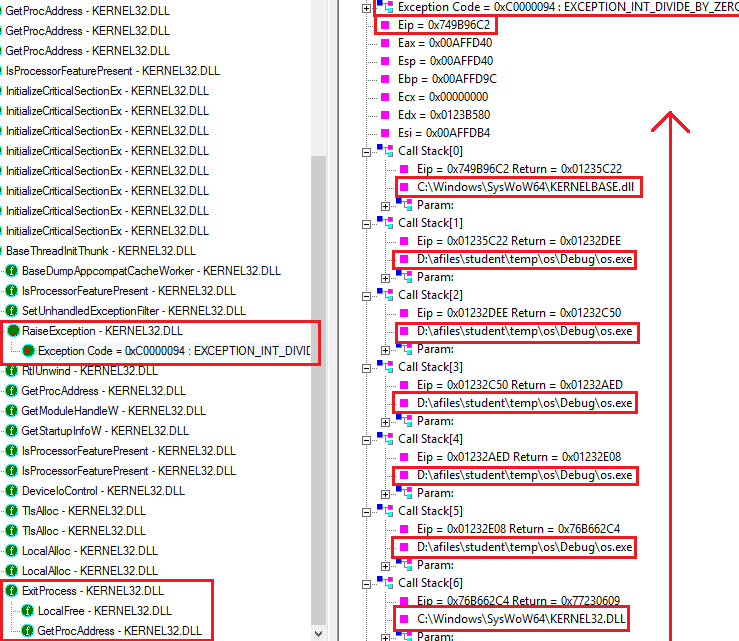
\includegraphics[scale = 0.70]{images/4.png}
	\caption{Состояние регистров процессора и стек вызовов}
\end{figure}

\subsection{Использовать функции UnhandleExceptionFilter и SetUnhandleExceptionFilter для необработанных исключений}

Помимо конструкции \_\_try и \_\_except в Windows имеется возможность превратить весь код в охраняемый, посредством установления фильтра на необработанные исключения. По большей части это считается плохим тоном, однако может быть полезно на стадии релиза приложения, когда при возникновении необработанной ошибки программа должна показывать диалоговое окно с ее описанием.

Установление фильтра на необработанные исключения производится функцией SetUnhandleExceptionFilter, которая имеет следующую сигнатуру [6]:

\begin{lstlisting}
LPTOP_LEVEL_EXCEPTION_FILTER WINAPI SetUnhandledExceptionFilter(
    _In_ LPTOP_LEVEL_EXCEPTION_FILTER lpTopLevelExceptionFilter
);
\end{lstlisting}

В качестве единственного аргумента принимается указатель на функцию фильтр. Возвращаемое значение содержит указатель на предыдущую функцию обработчик.

Разработаем программу, которая устанавливает фильтр необработанных исключений, выводит адрес старого фильтра, нового фильтра и после этого выбрасывает исключение.

\lstinputlisting{listings/5.cpp}

Результат работы программы:

\lstinputlisting{listings/5.log}

Рассмотрим системные вызовы, произведенные в этой программе. Перед запуском функции main операционная система сама устанавливает стандартный фильтра необработанных исключений.

\begin{figure}[h!]
	\centering
	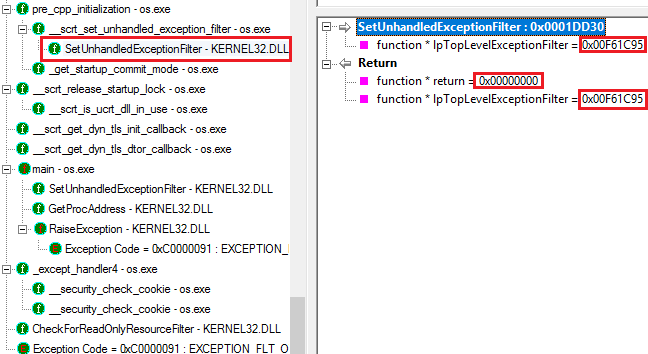
\includegraphics[scale = 0.92]{images/5_1.png}
	\caption{Установка стандартного фильтра необработанных исключений при запуске процесса}
\end{figure}

Стоит отметить, что адрес этой функции соответствует адресу, выведенному в результате выполнения программы (OLD\_EXCEPTION\_HANDLER). Возвращаемое значение этой функции является нулевым, потому что до этого не было установлено ни одного фильтра необработанных исключений.

После этого, уже в теле функции main, вызывается функция SetUnhandleExceptionFilter, которая была объявлена в программном коде:

\begin{figure}[h!]
	\centering
	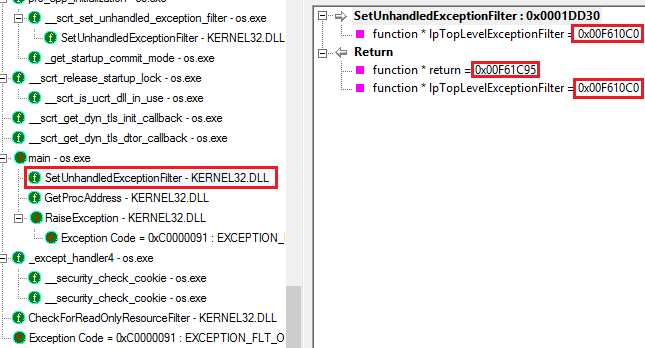
\includegraphics[scale = 0.92]{images/5_2.png}
	\caption{Установка собственного фильтра необработанных исключений}
\end{figure}

Адрес этой функции соответствует адресу, выведенному в результате выполнения программы (NEW\_EXC\linebreak EPTION\_HANDLER). Возвращаемое значение этой функции указывает на предыдущий фильтр, установленный операционной системой.

\subsection{Обработать вложенные исключения}

Архитектура обработки исключений в WinAPI позволяет обрабатывать вложенные блоки \_\_try, \_\_except. Для того, чтобы передать управление внешнему обработчику исключений из внутреннего, фильтр внутреннего обработчика должен возвращать EXCEPTION\_CONTINUE\_SEARCH.

Разработаем программу, которая содержит один блок \_\_try, \_\_except внутри другого. Внутренний обработчик вызывается на исключение EXCEPTION\_INT\_DIVIDE\_BY\_ZERO, в противном случае продолжит искать обработчик дальше. Внешний обработчик вызывается на исключение EXCEPTION\_FLT\_OVERFLOW, в противном случае продолжит искать обработчик дальше. Внутри охраняемого кода вызывается соответствующее исключение, в зависимости от аргумента командной строки.

\lstinputlisting{listings/6.cpp}

Результат работы программы:

\lstinputlisting{listings/6.log}

В первом варианте (аргумент 0 -- EXCEPTION\_INT\_DIVIDE\_BY\_ZERO) внутренний фильтр вернул EXCEPTION\_EXECUTE\_HANDLER после чего был вызван обработчик и приложение завершилось.

Во втором варианте (аргумент 1 -- EXCEPTION\_FLT\_OVERFLOW) внутренний фильтр вернул EXCEPTION\_CONTINUE\_SEARCH после чего был найден внешний обработчик. Внешний фильтр вернул EXCEPTION\_EXECUTE\_HANDLER, был вызван обработчик и приложение завершилось.

\clearpage

Рассмотрим обработку вложенного исключение более подробно на примере второго варианта (аргумент 1 -- EXCEPTION\_FLT\_OVERFLOW):

\begin{figure}[h!]
	\centering
	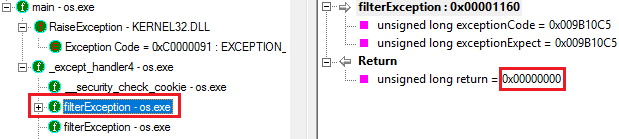
\includegraphics[scale = 0.85]{images/6_1.png}
	
	\caption{Вызов фильтра внутреннего обработчика}
	\label{image:6}
\end{figure}

Во внутреннем обработчике фильтр вернул 0 (EXCEPTION\_CONTINUE\_SEARCH).

\begin{figure}[h!]
	\centering
	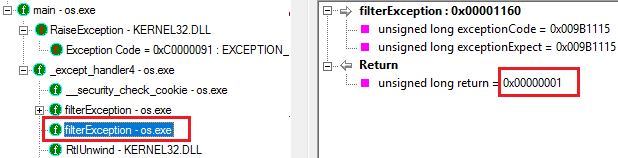
\includegraphics[scale = 0.85]{images/6_2.png}
	\caption{Вызов фильтра внешнего обработчика}
\end{figure}

Во внешнем обработчике фильтр вернул 1 (EXCEPTION\_EXECUTE\_HANDLER). Кроме того, раскрутка стека (RtlUnwind) была произведена только при нахождении обработчика (EXCEPTION\_EXECUTE\_HANDLER), при возвращении EXCEPTION\_CONTINUE\_SEARCH из внутреннего фильтра раскрутка стека не производится.

\subsubsection{Иллюстрация процесса обработки вложенных исключения в деассемблере Ida}

Рассмотрим процесс поиска обработчика для вложенных исключений с помощью деассембдера Ida для исключения 0xC0000091 EXCEPTION\_FLT\_OVERFLOW. После прохождения всех подготовительных стадий вызывается главная функция main, из которой вызывается внешняя функция ядра RaiseException с тремя нулевыми аргументами и кодом исключения:

\begin{figure}[h!]
	\centering
	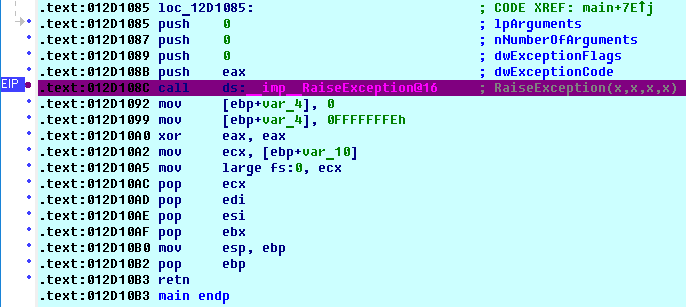
\includegraphics[scale = 0.75]{images/6_d1.png}
	\caption{Вызов внешней функции RaiseException из функции main}
\end{figure}

Стоит отметить, что последющий код функции main соответствует нормальному выходу из охраняемого кода, то есть случаю, когда исключение не сгенерируется. В нашем случае эта ветка кода не будет вызвана.

\clearpage

Как и следовало ожидать, было сгенерировано исключение EXCEPTION\_FLT\_OVERFLOW:

\begin{figure}[h!]
	\centering
	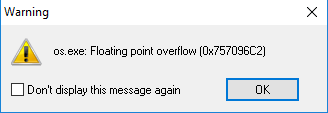
\includegraphics[scale = 0.75]{images/6_d2.png}
	\caption{Уведомление о произошедшем исключении}
\end{figure}

После этого мы попадаем в функцию except\_handler, что свидетельствует о том, что исключение было успешно выброшено и начался поиск обработчика:

\begin{figure}[h!]
	\centering
	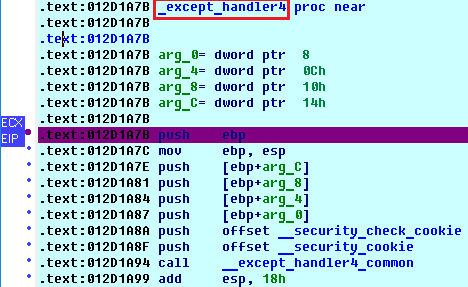
\includegraphics[scale = 0.75]{images/6_d3.png}
	\caption{Вызов функции except\_handler, предшествующей опросу фильтров}
\end{figure}

В первую очередь вызывается первый фильтр, который проверяет код исключения на совпадение с 0xC0000094 EXCEPTION\_INT\_DIVIDE\_BY\_ZERO:

\begin{figure}[h!]
	\centering
	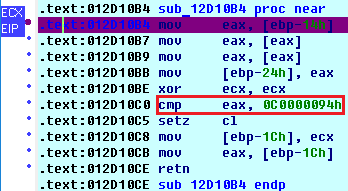
\includegraphics[scale = 0.95]{images/6_d4.png}
	\caption{}
\end{figure}

Код выброшенного исключения не совпадает с кодом фильтра, поэтому вызывается фильтр для следующего обработчика, который проверяет код исключения на совпадение с 0xC0000091 EXCEPTION\_FLT\_OVERFLOW:

\begin{figure}[h!]
	\centering
	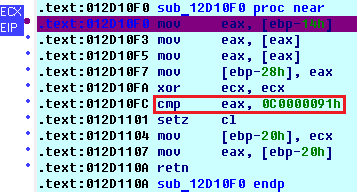
\includegraphics[scale = 0.75]{images/6_d5.png}
	\caption{}
\end{figure}

Фильтр сработал и обработчик был успешно найден, о чем свидетельствует последующий вызов функций раскрутки стека RtlUnwind в модулях ядра kernel32 и ntdll:

\begin{figure}[h!]
	\centering
	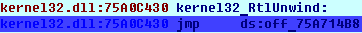
\includegraphics[scale = 0.75]{images/6_d6.png}
	\caption{Функция раскрутки стека RtlUnwind в модуле kernel32}
\end{figure}

\begin{figure}[h!]
	\centering
	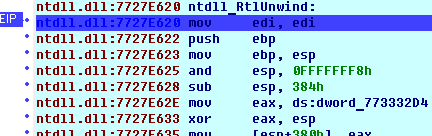
\includegraphics[scale = 0.75]{images/6_d7.png}
	\caption{Функция раскрутки стека RtlUnwind в модуле ntdll}
\end{figure}

Количество ассемблерных команд в RtlUnwind достаточно большое, что подтверждает ожидания. 

\subsection{Выйти из блока \_\_try с помощью оператора goto}

В WinAPI, а также в стандарте языка C++ разрешается выходить из охраняемого кода при помощи оператора goto. Использование оператора goto является плохой практикой в современных языках программирования, не только из-за абсолютного читабельности кода, но и из-за своей неэффективности. Каждый раз при использовании goto вызывается раскрутка стека, что делает данную операцию весьма медленной.

Однако, различные компиляторы языка C и C++ демонстрируют различное поведение ввиду внутренних оптимизаций. Например, компилятор GCC каждый раз раскручивает стек, в то время как MSVC от Microsoft добавляет оптимизацию выхода через goto из охраняемого кода, не раскручивая стек (скорее всего используется оптимизация через \_\_leave). Таким образом, для языка C goto ускоряется, а для языка C++ становится опасным, ведь нет гарантии вызова деструкторов для объектов охраняемого кода.

Разработаем программу, которая в зависимости от аргумента командной строки, выходит из охраняемого кода через goto или \_\_leave:

\lstinputlisting{listings/7.cpp}

Результат работы программы:

\lstinputlisting{listings/7.log}

Таким образом, goto позволил выйти из охраняемого кода. Раскрутка стека при этом не была вызвана ввиду внутренней оптимизации компилятора MSVC. Однако, goto по-прежнему считается не нормальным выходом из блока \_\_try, \_\_except, поэтому функция AbnormalTermination вернет 1.

\subsection{Выйти из блока \_\_try с помощью оператора \_\_leave}

В отличие от goto, команда \_\_leave позволяет выходить только из охраняемого кода. Использование \_\_leave в другом месте вызовет ошибку компиляции. Кроме того, \_\_leave не позволяет выходить из вложенных блоков \_\_try, \_\_except. Однако, использование этой команды рекомендуется при работе с исключениями, потому что не вызывает раскрутку стека, а также увеличивает читабельность кода [7]

Подадим на вход командной строки 0, для использования команды \_\_leave:

\lstinputlisting{listings/8.log}

Результат аналогичен goto, однако \_\_leave для всех компиляторов гарантированно не вызовет раскрутку стека.

\subsection{Преобразовать структурное исключение в исключение языка С, используя функцию translator}

Использовать одновременно исключения обоих типов, в программе на С++ проблематично, так как прийдется их обрабатывать по отдельности. Что-бы этого избежать SEH исключение нужно транслировать в обычное исключение. Делается это с помощью функции \_set\_se\_translator стандартной библиотеки, сама эта функция стандартной не является. Она получает указатель на функцию транслятор, которая получает структуру описывающую исключение и в ответ, должна бросить типизированное исключение.

Сигнатура функции \_set\_se\_translator выглядит следующим образом:

\begin{lstlisting}
_se_translator_function _set_se_translator(  
    _se_translator_function seTransFunction  
);  
\end{lstlisting}

Функция принимает на вход функцию транслятора и не возвращает значение. Функция транслятор принимает код структурного исключения и информацию о нем. Транслятор должен выбрасывать соответствующее исключение C++. Для того, чтобы компилятор MSVC разрешил использовать \_set\_se\_translator, обязательно использование флага компилятора /EHa [8]

Разработаем программу, которая транслирует структурное исключение, вызванное функцией RaiseException в исключение языка C++. При этом код исключения передается как указатель через throw:

\lstinputlisting{listings/9.1.cpp}

Результат работы программы:

\lstinputlisting{listings/9.1.log}

Доработаем программу, добавив возможность передачи структуры с информацией об исключении. Стоит отметить, что структуру нужно скопировать перед отправкой через throw, иначе она будет вычищена. 

\lstinputlisting{listings/9.2.cpp}

Результат работы программы:

\lstinputlisting{listings/9.2.log}

\subsection{Использовать финальный обработчик finally}

Помимо конструкции \_\_try, \_\_except поддерживается также конструкция \_\_try, \_\_finally. Блок \_\_finally был создан для задачи высвобождения ресурсов и будет вызван \textbf{в любом случае} после завершения охраняемого кода [9] Докажем это, разработаем программу, которая выходит из охраняемого кода пятью различными способами:

\lstinputlisting{listings/10.cpp}

Вне зависимости от способа выхода из охраняемого кода, блок \_\_finally должен выполняться. Результат работы программы для всех пяти способов:

\lstinputlisting{listings/10.log}

Таким образом блок \_\_finally был вызван во всех пяти различных вариантах. В данном примере не были рассмотрены варианты выхода через break и continue, но результаты аналогичны.

\subsection{Проверить корректность выхода из блока \_\_try с помощью функции AbnormalTermination в финальном обработчике}

Корректность выхода из охраняемого кода может повлиять на освобождение ресурсов в блоке \_\_finally. Для этого была создана функция AbnormalTermination, имеющая следующую сигнатуру [10]:

\begin{lstlisting}
BOOL AbnormalTermination(void);
\end{lstlisting}

Функция возвращает 0, если завершение нормальное и 1, если нет. Данная функция может быть вызвана только из блока \_\_finally.

Корректным выходом из охраняемого кода считается самостоятельное завершение и команда \_\_leave. Все остальные варианты выхода являются не нормальным завершением и должны вызывать раскрутку стека. Однако, MSVC от Microsoft добавляет оптимизацию выхода из охраняемого кода, не раскручивая стек (скорее всего используя \_\_leave), что ускоряет работу кода, но паразитно для проведения экспериментов. Тем не мение, AbnormalTermination работает правильно, согласно спецификации.

Дополним программу из предыдущего пункта, добавив обработку нормального и не нормального завершения в блок \_\_finally:

\lstinputlisting{listings/11.cpp}

Результат работы программы:

\lstinputlisting{listings/11.log}

Только в первых двух случаях (самостоятельное завершение и команда \_\_leave) охраняемый код завершился нормально, в то время как в остальных случаях завершение было не нормальным.

\clearpage

\section{Вывод}

В результате работы были изучены структурные исключения SEH. Из преимуществ данного способа обработки исключений, по сравнению со встроенными средствами языка C++ является:

\begin{itemize}
	\item возможность обработки аппаратных исключений и просмотра регистров процессора на момент их возникновения;
	\item поддерживаются как в языке C, так и в C++;
	\item возможность транслирования исключений в исключения языка C++.
\end{itemize}

Из минусов стоит отметить:

\begin{itemize}
	\item зависимость от конкретной платформы, в то время как исключения языка C++ стандартизованы.
\end{itemize}

Кроме того, не стоит забывать, что раскрутка стека является достаточно трудоемкой операцией, поэтому программист должен отдавать себе отчет в том, какие операции вызывают нормальное завершение охраняемого кода, а какие нет. Стоит отметить, что иногда компилятор может встроить дополнительную оптимизацию, для того чтобы не раскручивать стек в таких ситуациях, однако, такие улучшения обычно не стандартизированы, не надежны и тяжело отслеживаются на этапе отладки.

\section{Список литературы}

\begin{flushleft}

[1] Эксплуатирование SEH в среде Win32 [Электронный ресурс]. — URL: \href{http://www.securitylab.ru/contest/212085.php}{http://www.securitylab.ru/contest/212085.php} (дата обращения 05.10.2017).
\linebreak
	
[2] ОБРАБОТКА ИСКЛЮЧЕНИЙ В VISUAL C++ [Электронный ресурс]. — URL: \href{http://www.avprog.narod.ru/progs/exceptions.htm}{http://www.avprog.narod.ru/progs/exceptions.htm} (дата обращения 05.10.2017).
\linebreak
	
[3] Раскрутка стека. C++ для начинающих [Электронный ресурс]. — URL: \href{https://it.wikireading.ru/35947}{https://it.wikireading.ru/35947} (дата обращения 05.10.2017).
\linebreak
	
[4] EXCEPTION\_RECORD structure (Windows) [Электронный ресурс]. — URL: \href{https://msdn.microsoft.com/ru-ru/library/windows/desktop/aa363082(v=vs.85).aspx}{https://msdn.microsoft.com/ru-ru/library/windows/desktop/aa363082(v=vs.85).aspx} (дата обращения 05.10.2017).
\linebreak
	
[5] RaiseException function (Windows) [Электронный ресурс]. — URL: \href{https://msdn.microsoft.com/ru-ru/library/windows/desktop/ms680552(v=vs.85).aspx}{https://msdn.microsoft.com/ru-ru/library/windows/desktop/ms680552(v=vs.85).aspx} (дата обращения 05.10.2017).
\linebreak
	
[6] SetUnhandledExceptionFilter function (Windows) [Электронный ресурс]. — URL: \href{https://msdn.microsoft.com/ru-ru/library/windows/desktop/ms680634(v=vs.85).aspx}{https://msdn.microsoft.com/ru-ru/library/windows/desktop/ms680634(v=vs.85).aspx} (дата обращения 05.10.2017).
\linebreak
	
[7] Оператор try-except [Электронный ресурс]. — URL: \href{https://msdn.microsoft.com/ru-ru/library/s58ftw19.aspx}{https://msdn.microsoft.com/ru-ru/library/s58ftw19.aspx} (дата обращения 05.10.2017).
\linebreak
	
[8] Очень серьезный блог: Обработка исключений и корректность программ на С++. [Электронный ресурс]. — URL: \href{http://evgeny-lazin.blogspot.ru/2008/07/blog-post.html}{http://evgeny-lazin.blogspot.ru/2008/07/blog-post.html} (дата обращения 05.10.2017).
\linebreak
	
[9] Оператор try-finally [Электронный ресурс]. — URL: \href{https://msdn.microsoft.com/ru-ru/library/9xtt5hxz.aspx}{https://msdn.microsoft.com/ru-ru/library/9xtt5hxz.aspx} (дата обращения 05.10.2017).
\linebreak
	
[10] AbnormalTermination macro (Windows) [Электронный ресурс]. — URL: \href{https://msdn.microsoft.com/ru-ru/library/windows/desktop/ms679265(v=vs.85).aspx}{https://msdn.microsoft.com/ru-ru/library/windows/desktop/ms679265(v=vs.85).aspx} (дата обращения 05.10.2017).
\linebreak

\end{flushleft}

\end{document}